\section{Auswertung}
\label{sec:Auswertung}
Die direkt an der Monozelle abgegriffene Leerlaufspannung $U_\text{0}$ ergibt sich etwa zu $1.5 \si{\ohm}$.
Der Fehler des Voltmeters beträgt nach Herstellerangaben im verwendeten Messbereich $1.5\%$.
Damit ergibt sich $U_\text{0}=(1.5 \pm 0.0225) \si{\ohm}$.
Der Innenwiderstand des Voltmeters ist nach Herstellerangaben $R_\text{V}\approx 10 \cdot 10^6 \si{\ohm}$.

Der Innenwiderstand $R_\text{i}$ und die Leerlaufspannung $U_\text{0}$ der Monozelle ergeben sich mit Linearer Regression nach \eqref{eqn:ausgleichsgrade} unter Verwendung von Formel ???.
Dazu werden die in Tabelle \ref{tab:monozelle} gelisteten $U_\text{k}$ gegen $I$ aufgetragen.
\begin{equation*}
  -a= R_\text{i}=(15.5\pm0.3)\si{\ohm}
\end{equation*}
\begin{equation*}
  b =U_\text{0}=(1501.4\pm13.9)\si{\milli\volt}
\end{equation*}


\begin{table}
  \centering
  \label{tab:monozelle}
  \caption{Messdaten für die Klemmenspannung in Abhängigkeit des Strom bei der Monozelle}
\begin{tabular}{cc}
  \toprule
$U_\text{k}$/$\si{\milli\volt}$ & $I$/$\si{\milli\ampere}$\\
\midrule
69.0 & 91.0 \\
342.0 & 74.0 \\
550.0 & 61.0 \\
700.0 & 52.0 \\
825.0 & 45.0 \\
910.0 & 40.0 \\
965.0 & 37.0 \\
980.0 & 35.0 \\
990.0 & 32.0 \\
1026.0 & 30.0 \\
1056.0 & 28.0 \\
1083.0 & 26.0 \\
1110.0 & 24.0 \\
1116.0 & 23.0 \\
\bottomrule
\end{tabular}
\end{table}
\begin{figure}
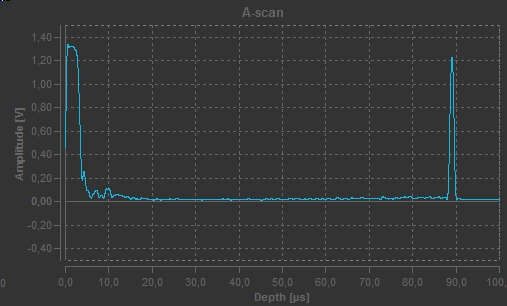
\includegraphics{Bilder/a.pdf}
\caption{Linearer Fit zur Monozelle ohne Gegenspannung}
\label{fig:plot_a}
\end{figure}


%monozelle belastet
\begin{equation*}
  a= R_\text{i}=(17.3\pm 0.5)\si{\ohm}
\end{equation*}
\begin{equation*}
  b =U_\text{0}=(1626.3\pm 26.1)\si{\milli\volt}
\end{equation*}
\begin{table}
  \centering
  \label{tab:monozelle_belastet}
  \caption{Messdaten für die Klemmenspannung in Abhängigkeit des Strom bei der Monozelle mit Gegenspannung}
\begin{tabular}{cc}
  \toprule
$U_\text{k}$/$\si{\milli\volt}$ & $I$/$\si{\milli\ampere}$\\
\midrule
3400.0 & 99.0 \\
3100.0 & 92.0 \\
2850.0 & 68.0 \\
2700.0 & 58.0 \\
2460.0 & 49.0 \\
2340.0 & 42.0 \\
2250.0 & 37.0 \\
2160.0 & 33.0 \\
2100.0 & 29.0 \\
2070.0 & 26.0 \\
2040.0 & 24.0 \\
2010.0 & 21.0 \\
1980.0 & 20.0 \\
1970.0 & 19.0 \\
\bottomrule
\end{tabular}
\end{table}
\begin{figure}
\includegraphics{Bilder/c.pdf}
\caption{Linearer Fit zur Monozelle mit Gegenspannung}
\label{fig:plot_monozellebelastet}
\end{figure}



%rechteckspannung
\begin{equation*}
  -a= R_\text{i}=(69.1\pm0.7)\si{\ohm}
\end{equation*}
\begin{equation*}
  b =U_\text{0}=(477.8\pm1.4)\si{\milli\volt}
\end{equation*}

\begin{table}
  \centering
  \label{tab:reckteck}
  \caption{Messdaten für die Klemmenspannung in Abhängigkeit des Strom bei der Rechteckspannungsquelle}
\begin{tabular}{cc}
  \toprule
$U_\text{k}$/$\si{\milli\volt}$ & $I$/$\si{\milli\ampere}$\\
\midrule
165.0 & 4.5 \\
195.0 & 4.1 \\
245.0 & 3.4 \\
295.0 & 2.6 \\
325.0 & 2.2 \\
345.0 & 1.9 \\
365.0 & 1.7 \\
380.0 & 1.4 \\
395.0 & 1.2 \\
405.0 & 1.1 \\
415.0 & 1.0 \\
420.0 & 0.8 \\
425.0 & 0.7 \\
430.0 & 0.68 \\
430.0 & 0.67 \\
\bottomrule
\end{tabular}
\end{table}
\begin{figure}
\includegraphics{Bilder/d.pdf}
\caption{Linearer Fit zur Rechteckspannung}
\label{fig:plot_rechteck}
\end{figure}



%sinusspannung
\begin{equation*}
  -a= R_\text{i}=(657.0± 5.0)\si{\ohm}
\end{equation*}
\begin{equation*}
  b =U_\text{0}=(1567.4\pm3.6)\si{\milli\volt}
\end{equation*}

\begin{table}
  \centering
  \label{tab:sinus}
  \caption{Messdaten für die Klemmenspannung in Abhängigkeit des Strom bei der Sinusspannungsquelle}
\begin{tabular}{cc}
  \toprule
$U_\text{k}$/$\si{\milli\volt}$ & $I$/$\si{\milli\ampere}$\\
\midrule
510.0 & 1.62 \\
675.0 & 1.35 \\
960.0 & 0.93 \\
1125.0 & 0.66 \\
1230.0 & 0.51 \\
1320.0 & 0.36 \\
1395.0 & 0.27 \\
1425.0 & 0.21 \\
1455.0 & 0.18 \\
1485.0 & 0.15 \\
1491.0 & 0.12 \\
1500.0 & 0.09 \\
\bottomrule
\end{tabular}
\end{table}
\begin{figure}
\includegraphics{Bilder/e.pdf}
\caption{Linearer Fit zur Sinusspannung}
\label{fig:plot_sinus}
\end{figure}
